\newpage

\subsection{QuizziPedia::Front-End::Directives}

\subsubsection{Informazioni generali}
\label{QuizziPedia::Front-End::Directives}
\begin{figure} [ht]
	\centering
	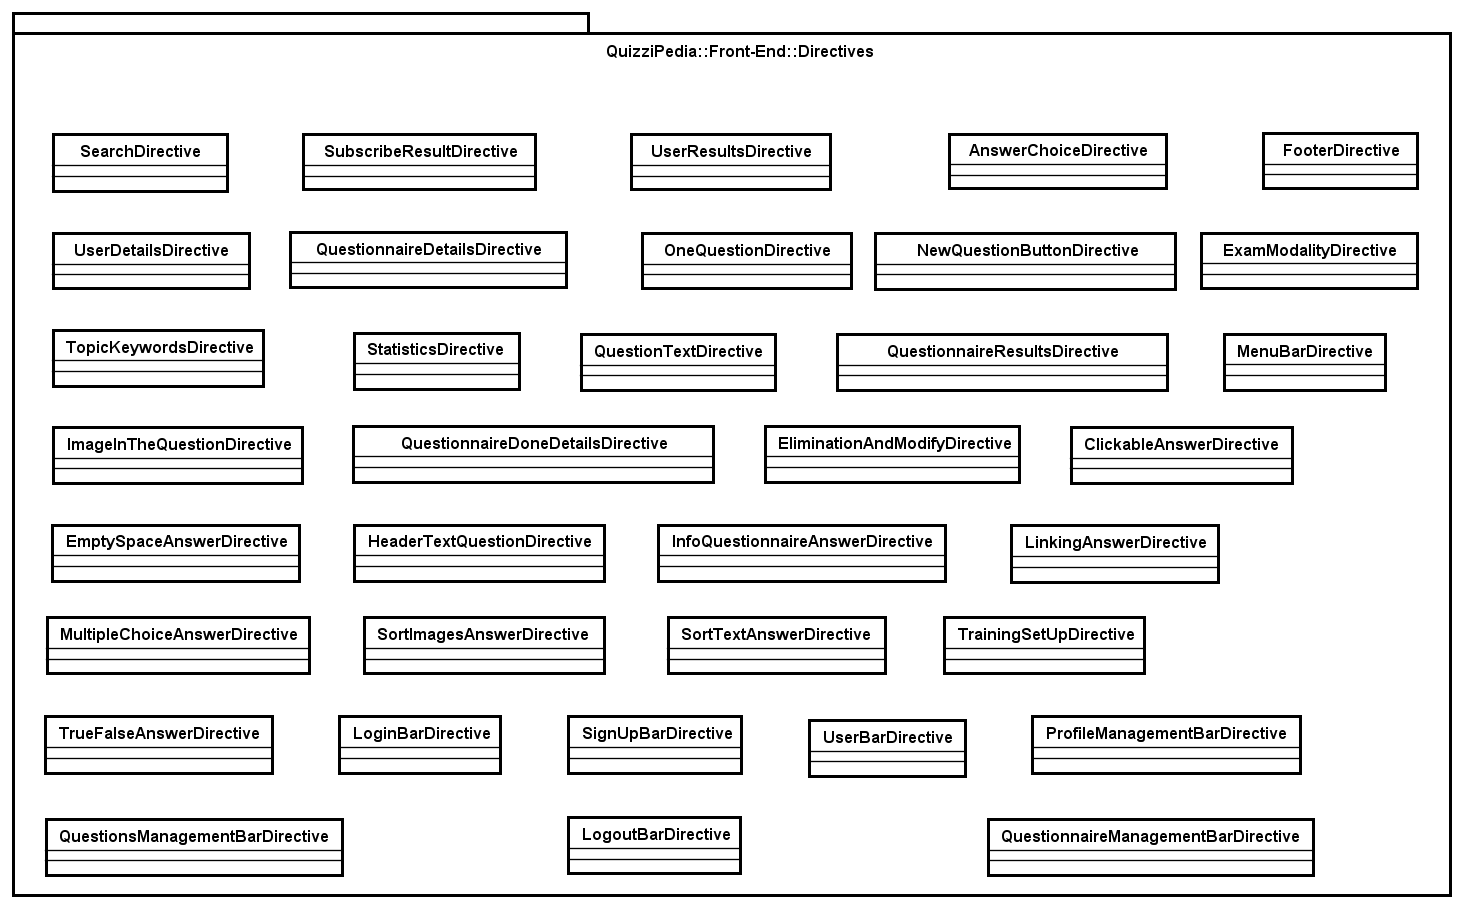
\includegraphics[scale=0.40]{UML/Package/QuizziPedia_Front-End_Directives.png}
	\caption{QuizziPedia::Front-End::Directives}
\end{figure}
\begin{itemize}
	\item \textbf{Descrizione}: package contenente le \textit{directives\ped{G}};
	\item \textbf{Padre}: \texttt{Front-End};
	\item \textbf{Interazione con altri componenti}:
	\begin{itemize}
		\item \texttt{Controllers}: package contenente i \textit{controllers\ped{G}} front-end dell'applicazione;
		\item \texttt{Views}: package contenente le \textit{views\ped{G}} front-end dell'applicazione.
	\end{itemize}
	\item \textbf{Classe contenute}:
	\begin{itemize}
		\item \texttt{EliminationAndModifyDirective}: componente grafico contenente i bottoni per eliminare o modificare un questionario;
		\item \texttt{ExamModalityDirective}: classe contenete i componenti grafici per attivare la modalità esame su un questionario e gestire le iscrizioni;
		\item \texttt{FooterDirective}: classe contenente i componenti grafici del footer dell'applicazione;
		\item \texttt{ImageInTheQuestionDirective}: classe contenente i componenti grafici per l'inserimento dell'immagine	nella creazione delle domande;
		\item \texttt{MenuBarDirective}: rappresenta il menù, presente in ogni pagina dell'applicazione, generato in base agli oggetti passati nello \$scope isolato. Fornisce un pulsante per ogni oggetto ricevuto come parametro, ogni pulsante viene rappresentato con un'icona e con un testo. Al click di un pulsante viene invocata la funzione ad esso associata;
		\item \texttt{OneQuestionDirective}: rappresenta il componente grafico che visualizza all'utente l'anteprima della domanda che ha creato. Eseguendo l'azione di click sul pulsante di modifica sarà possibile modificare tale domanda. All'interno di QuestionsManagementsView verranno stampati a video tanti componenti quanti presenti nello \$scope isolato ad esso associato;
		\item \texttt{NewQuestionButtonDirective}: rappresenta il componente grafico che permette all'utente di posizionarsi nella \textit{view\ped{G}} di creazione di una nuova domanda;
		\item \texttt{QuestionTextDirective}: rappresenta il componente grafico che permette all'utente di scrivere o modificare il testo di una domanda;
		\item \texttt{QuestionnaireDetailsDirective}: rappresenta il componente grafico che permette all'utente di visualizzare la lista di questionari che può compilare;
		\item \texttt{QuestionnaireDoneDetailsDirective}: rappresenta il componente grafico che permette all'utente di visualizzare la lista di questionari che ha già compilato e di conseguenza vederne le valutazioni;
		\item \texttt{}: rappresenta il componente grafico che permette all'utente autenticato pro di vedere i risultati di chi ha compilato il questionario. Tale componente è contenuto nella lista dei questionari abilitati alla compilazione. É possibile accedere alla lista dei risultati azionando l'evento ad esso collegato;
		\item \texttt{QuestionnaireResultsDirective}: rappresenta il componente grafico che permette all'utente autenticato pro di vedere i risultati di chi ha compilato il questionario. Tale componente è contenuto nella lista dei questionari abilitati alla compilazione. É possibile accedere alla lista dei risultati azionando l'evento ad esso collegato;
		\item \texttt{SearchDirective}: classe che permette di effettuare la ricerca di utenti e questionari;
		\item \texttt{StatisticsDirective}: classe che permette di visualizzare le statistiche di un utente;
		\item \texttt{SubscribeResultDirective}: classe che permette di visualizzare e iscriversi ai questionari ricercati;
		\item \texttt{TopicKeywordsDirective}: classe che permette di gestire l'inserimento dell'argomento e delle	keywords al momento della creazione della domanda;
		\item \texttt{UserDetailsDirective}: classe che permette di visualizzare i dati personali di un utente;
		\item \texttt{UserResultsDirective}: classe che permette di visualizzare la lista degli utenti ricercati dopo aver utilizzato l'apposita funzione di ricerca;
		\item \texttt{ClickableAnswerDirective}: rappresenta il componente grafico che permette all'utente di visualizzare la domanda ad area cliccabile nell'immagine;
		\item \texttt{EmptySpaceAnswerDirective}: rappresenta il componente grafico che permette all'utente di visualizzare l'esercizio a riempimento di spazi vuoti;
		\item \texttt{}:
		\item \texttt{}:
		\item \texttt{}:
		\item \texttt{}:
		\item \texttt{}:
		\item \texttt{}:
		\item \texttt{}:
		\item \texttt{}:
		\item \texttt{}:
		\item \texttt{}:
		\item \texttt{}:
		\item \texttt{}:
		\item \texttt{}:
		\item \texttt{}:	
	\end{itemize}
\end{itemize}